%% $RCSfile: proj_proposal.tex,v $
%% $Revision: 1.2 $
%% $Date: 2010/04/23 02:40:16 $
%% $Author: kevin $

\documentclass[11pt, a4paper, twoside, openright, notitlepage]{report}

\usepackage{float} % lets you have non-floating floats

\usepackage{url} % for typesetting urls

%  We don't want figures to float so we define
%
\newfloat{fig}{thp}{lof}[chapter]
\floatname{fig}{Figure}

%% These are standard LaTeX definitions for the document
%%
\title{Web Application Key Management Progress Report}
\author{Sriram Venkatesh}

%% This file can be used for creating a wide range of reports
%%  across various Schools
%%
%% Set up some things, mostly for the front page, for your specific document
%
% Current options are:
% [ecs|msor]              Which school you are in.
%
% [bschonscomp|mcompsci]  Which degree you are doing
%                          You can also specify any other degree by name
%                          (see below)
% [font|image]            Use a font or an image for the VUW logo
%                          The font option will only work on ECS systems
%
\usepackage[image,ecs]{vuwproject} 

% You should specifiy your supervisor here with
%     \supervisor{Firstname Lastname}
% use \supervisors if there are more than one supervisor

% Unless you've used the bschonscomp or mcompsci
%  options above use
\otherdegree{Bachelor of Engineering}
% here to specify degree

\supervisors{Dr Ian Welch, Michael Gannon,  Nick Clarke, Dr Kris Bubendorfer}


% Comment this out if you want the date printed.
\date{}

\begin{document}

% Make the page numbering roman, until after the contents, etc.
\frontmatter

%%%%%%%%%%%%%%%%%%%%%%%%%%%%%%%%%%%%%%%%%%%%%%%%%%%%%%%

\begin{abstract}
The objective of this report is describe and demonstrate the progress of the Web Application Key Management project and develop a plan for the remainder of the project. The project looks at how applications can manage encrypted credential keys for secure web applications. The project is split into two phases, where we look into the traditional case and also a modern case into the cloud. The literature review conducted finds there have been various attempts to solve the issue. This report looks at a comparative view of the best option by comparing various threat models and abstractions. 
\end{abstract}

%%%%%%%%%%%%%%%%%%%%%%%%%%%%%%%%%%%%%%%%%%%%%%%%%%%%%%%

\maketitle

%\tableofcontents

% we want a list of the figures we defined
%\listof{fig}{Figures}

%%%%%%%%%%%%%%%%%%%%%%%%%%%%%%%%%%%%%%%%%%%%%%%%%%%%%%%

\mainmatter

%%%%%%%%%%%%%%%%%%%%%%%%%%%%%%%%%%%%%%%%%%%%%%%%%%%%%%%

\section*{1 Introduction}
As the web becomes increasingly complex, web applications become more complicated and dynamic. Web pages are no longer static; they contain dynamic content from many different external sources. To access these external services, the web application is configured with credentials to gain access to those systems - for example, username/passwords, certificates or API Keys. \\



requires credentials to access these systems, such as API Keys, Username and Passwords and certificates which are stored on the server. \\

Howev

Sriram
Web applications require credentials to access these external systems.  








\section*{2 Literature Review}
\subsection*{2.1 Related Work}
Many credential management systems have been developed in order to protect and secure the valuable credential data. 


 of the research conducted in this project has been about addressing the problem of Key Management and how we can securely mange our credential data for the external systems. 


\subsubsection*{2.2.1 PKI}
\subsubsection*{2.2.1 Trust Management System}
A trust management system provides a standard, general-purpose mechanism for specifying application security polices and credentials  \cite{blaze1999keynote}. Trust management systems were devised as a alternative to Access Control Lists (ACL). An ACL, is a list of permissions attached to an object. It will specify what users, or system processes are granted access to objects, and also specify what operations are allowed on given objects. \cite{acl-rfc} \\



 to Security credentials allow applications to specify a delegation of trust among public keys. A trust management credential binds public keys to the authorization to perform specific tasks such as connecting to a database. \cite{blaze1999keynote}
\subsubsection*{2.1.2 KeyNote}
KeyNote is a 
\subsubsection*{2.1.3 PERMIS}
\subsubsection*{2.1.4 TPL}
\subsubsection*{2.1.5 Kerberos}



\section*{3 Project Progress}
\subsection*{3.1 Description of the Current Model}
Given a 



\subsection*{3.2 Decoupling the Application}
Before defining a solution to the problem, its important to define and construct a threat model to model the application. Decomposing the application is concerned with gaining an understanding of the application and how it interacts with external entities. This involves the applying the following steps to model the application:  

\begin{itemize}
  \item Create use cases to understand how the application is used.
  \item Identify the Entry Points to see where a potential attacker could interact with the application.
  \item Identify Assets that the attacker would be interested in.
  \item Identify assumptions for the components of the application, that an attacker would be interested in.
  \item Identify trust levels which represent the access rights the application with grant to external entities. 
\end{itemize}

Our simple abstracted application has one external dependency, being the external MySQL database.  The MySQL database requires the web application to be configured with credentials to access it. 

\begin{figure}[!ht]
    \centering
    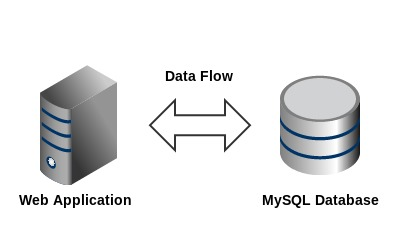
\includegraphics[width=0.5\textwidth]{external-overview.jpg}
    \caption{Connection between application and database}
\end{figure}

To connect to this database using JDBC, you will use the following Java method to pass in important authentication data to authorize access to the data store. At runtime the application requires the username and password pair in \emph{plain-text}. 


\begin{figure}[!ht]
\begin{lstlisting}
  Connection conn = DriverManager.getConnection(url, "username", "password");
\end{lstlisting} 
\caption{Java constructor for connecting to Database}
\end{figure}

For our simple case, we have stored the password in \emph{plain-text} in the configuration file. This password is required at runtime to ensure the connection between the web application and database is made. \\

\begin{figure}[!ht]
    \centering
    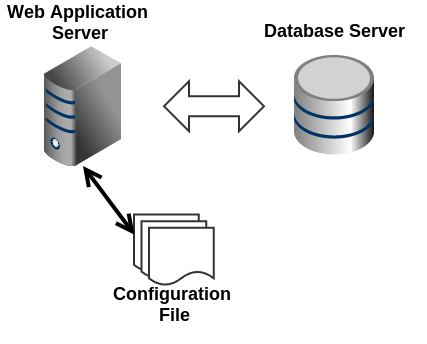
\includegraphics[width=0.5\textwidth]{config}
    \caption{Connection between application, database and configuration file}
\end{figure}

These credentials are stored in the hard disk and the web application is required to make various system calls to get the information. Our application is made of various internal components that are involved with the credential  information that we want to protect. In Figure 4 we can see the high level architectural view of the web application of the involved components. 

\begin{figure}[h!]
    \centering
    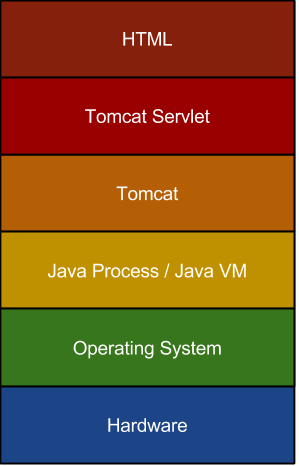
\includegraphics[height=0.2\paperheight]{high-level-archecuture}
    \caption{High Level Architectural View of the System}
\end{figure}

\subsection*{3.3 Entities of the Application}


\subsection*{3.4 Interaction Between Components}
\subsubsection*{3.4.1 Running Application}
The running application requires the \emph{plain-text} password for the connection to occur. The following steps occur during the runtime of the application to obtain the \emph{plain-text} password from the file on disk. 

\begin{enumerate}
\item The Java code is executed and gets to the line
\begin{lstlisting}
  Connection conn = DriverManager.getConnection(url, "username", "password");
\end{lstlisting}
This is is executed when the tomcat instance runs the complied servlet code.
\item Java instance makes a request to the OS for the cleat text password required for logging into the database
\item The operating system finds the location of the file and verifies whether the calling process is allowed access to the file.
\item Once, the operating system verifies the process, the operating system will obtain a copy of the configuration file on disk and put into memory for the Java process to access.
\item The java process will process the reference in memory of the configuration file and extract the password required to connect to the datastore.
\end{enumerate}

\begin{figure}[h!]
    \centering
    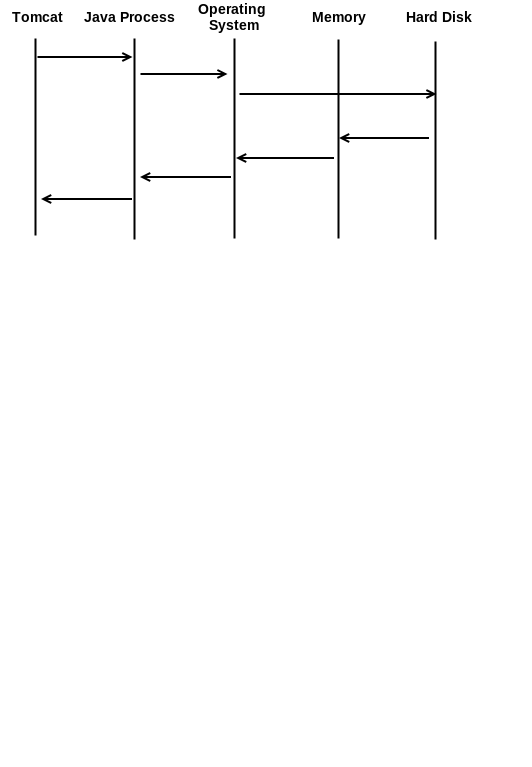
\includegraphics[height=0.2\paperheight]{sequence_diagram}
    \caption{Diagram of Sequence between entities.}
\end{figure}





\subsection*{3.5 Threat Scenarios}





\section*{4 Future Plans}





\section*{5 Feedback Required}






%%%%%%%%%%%%%%%%%%%%%%%%%%%%%%%%%%%%%%%%%%%%%%%%%%%%%%%
\backmatter
%%%%%%%%%%%%%%%%%%%%%%%%%%%%%%%%%%%%%%%%%%%%%%%%%%%%%%%

\bibliographystyle{ieeetr}
%\bibliographystyle{acm}
\bibliography{bib}
\end{document}
